\chapter{Conclusioni}\label{ch:conclusioni}
\section{Cosa ha funzionato bene}
Il lavoro che è stato descritto in questo elaborato di tesi può essere ritenuto soddisfacente.
\\Avendo infatti come punto di partenza \cite{soccerNet} in cui venivano effettuati esperimenti analoghi a quelli effettuati da noi nel nostro elaborato di tesi, siamo riusciti mediante l'uso di reti neurali ricorrenti ad ottnere, nel task di classififazione, risultati persino migliori
\\In tale task infatti siamo passati da una mAP del\textbf{ 67.8\%}, ottenuta nel sovracitato paper grazie al metodo di pooling \textbf{netVLAD}, ad una mAP del \textbf{79.7\%} ottenuta grazie all'utilizzo di \textbf{reti neurali ricorrenti}.
\\Successivamente ci siamo spinti oltre, infatti siamo passati dal task di classificazione a quello di localizzazione, questo è stato possibile grazie ad un processamento del dataset con un meccanismo di sliding windows.
\\Alla fine è stata inoltre decritta la procedura di generazione degli highlights, la quale era la naturale conclusione del nostro lavoro.
\section{Cosa ha funzionato meno bene}
Durante la fase di training, per cercare di ridurre gli effetti negativi dovuti al dataset fortementi sbilanciato, si è provato a usare una tecnica di \textbf{Data Augmentation}.
\\La nostra applicazione di tale tecnica è stata utilizzata per moltiplicare i campioni di ogni evento, questo è stato possibile anche qua mediante un meccanismo di \textbf{sliding-windows}.
\\Questi ulteriori campioni vengono aggiunti poi al dataset, aiutando a risolvere lo sbilanciamento di quest'ultimo.
\\I risultati applicando questa tecnica non sono stati tuttavia soddisfacenti, infatti le prestazioni della rete neurale si sono rivelate peggiori rispetto al modello che non ha fatto uso di \textbf{Data Augmentation}.\\
\\Nella figura \ref{figure : fakecard} abbiamo un esempio di \textbf{malfunzionamento} della rete neurale , infatti in tale figura vediamo come l'inquadratura \textbf{in primo piano} dell'aribtro induca la nostra rete neurale a pensare che sia stato estratto un \textbf{cartellino}, quando invece il giocatore è stato richiamato solo \textbf{verbalmente}.
\begin{figure}[ht]
\centering
\caption{Visualizzazione di un cartellino non correttamente predetto}
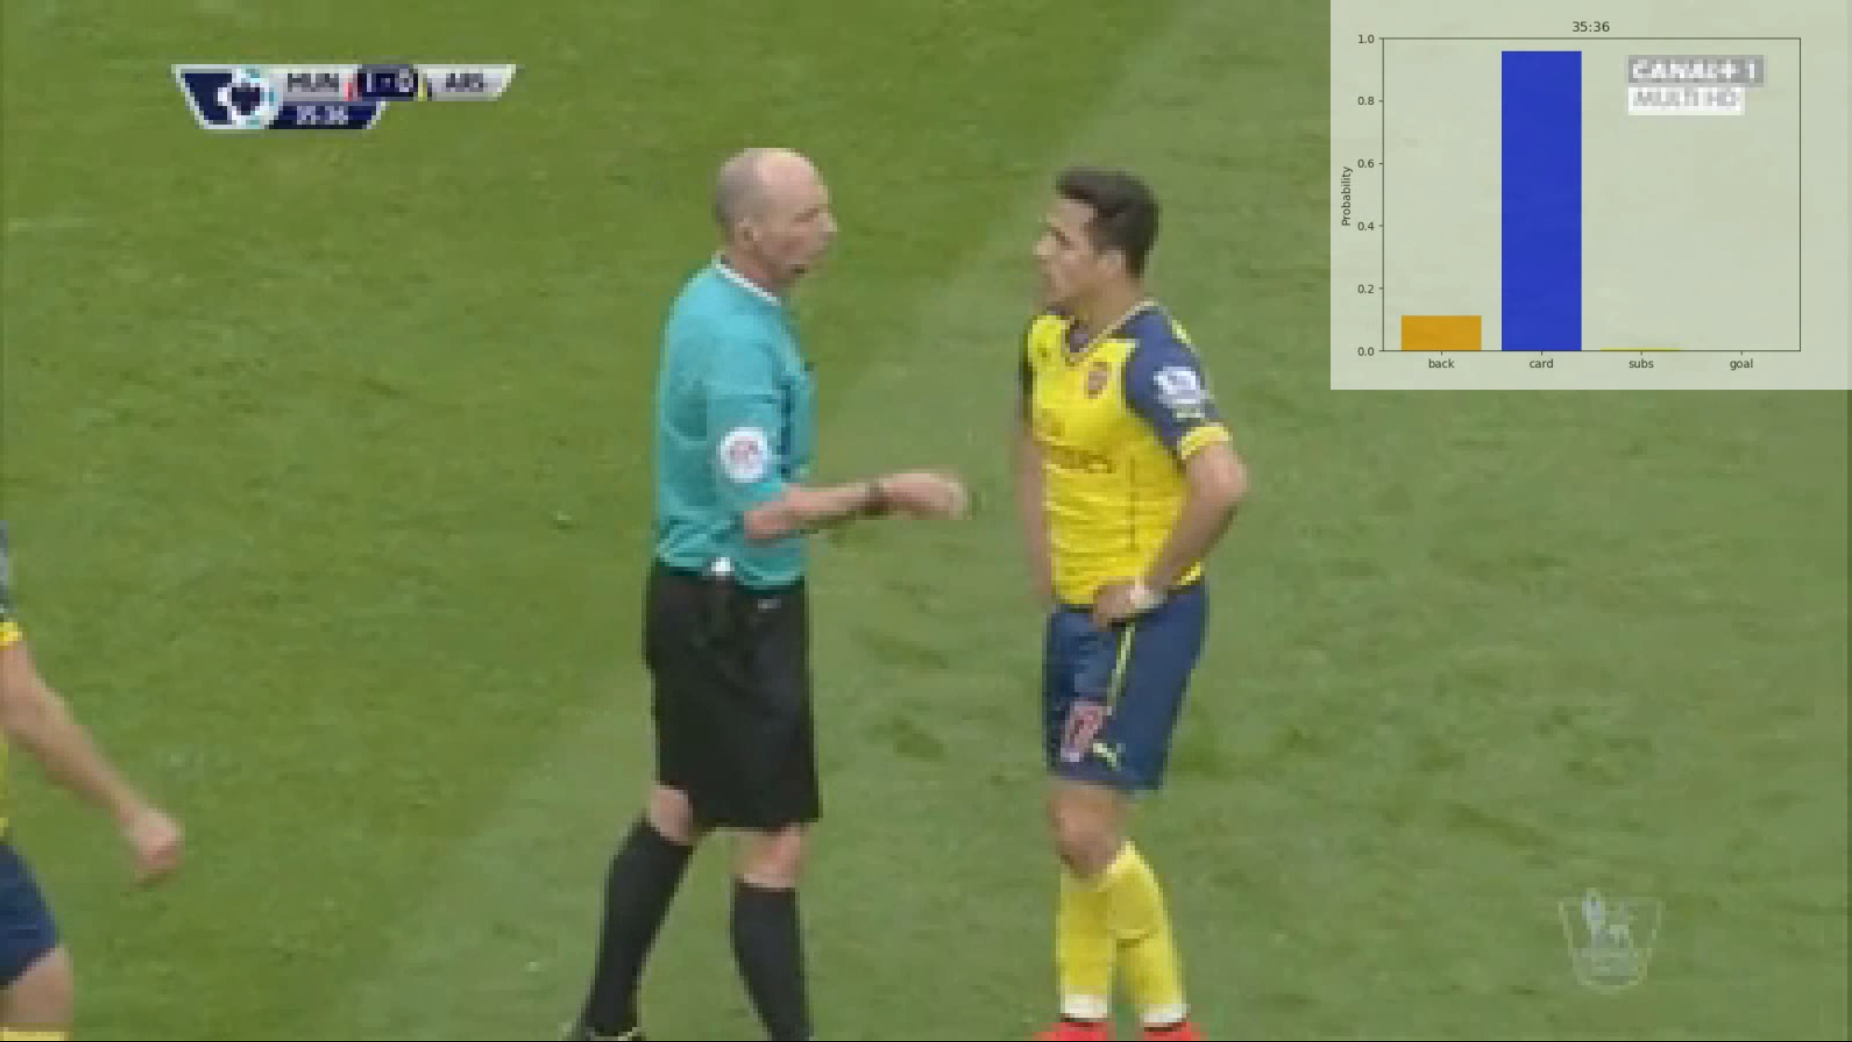
\includegraphics[width=\linewidth]{img/fakecard.png}
\label{figure : fakecard}
\end{figure}
\section{Lavoro futuro}
La naturale evoluzione di questo elaborato di tesi è quella di cercare di individuare altre tipologie di azioni oltre alle tre già prese in considerazione, ad esempio si potrebbero ricercare tiri in porta, calci d'angolo o calci di rigore.
\\Inoltre come citato nel paper \citep{soccerNet}, nell'estrazione delle features non è stato preso in considerazione l'audio, presente invece nei video originali.
\\Indubbiamente esso aggiunge informazioni significative e potrebbe essere d'aiuto ai nostri scopi, tuttavia come ben sappiamo l'audio non è sempre strettamente collegato a ciò che accade in campo, ma dipende da altri fattori quali: squadra di casa, momento della partita, affluenza di pubblico allo stadio\ldots
\\Questo fatto potrebbe confondere la rete neurale, portando ad un peggioramento delle prestazioni.
\\Rimane impossibile quindi esperimersi a \textbf{priori} su un possibile aiuto dell'audio nell'addestramento della rete neurale.
